\documentclass[11pt, a4paper, oneside]{article}

\usepackage[T1]{fontenc}
%\usepackage[utf8]{inputenc}
%\usepackage[english, polish]{babel}
\usepackage{polski}
\usepackage{setspace}
\usepackage{indentfirst}

\usepackage[left=2.0cm, right=2.0cm, top=1.5cm, bottom=2cm]{geometry}

\usepackage{fancyhdr}
\usepackage[table]{xcolor}
\usepackage{graphicx}
\usepackage{amsmath}
\usepackage{amsthm,thmtools}
\usepackage[nottoc]{tocbibind}
\usepackage{ragged2e}
\usepackage{bbding}
\usepackage{makeidx}
\usepackage{titlesec}
\usepackage{tcolorbox}
\usepackage{url}
\usepackage{color}
\usepackage{setspace}
\usepackage[font=small,format=plain,labelfont=bf,up,textfont=it,up]{caption}
\usepackage{BeamerColor}
\usepackage{listings}

\definecolor{mycolor1}{RGB}{0,0,128}
\definecolor{lightgray}{gray}{0.9}
\definecolor{lightlightgray}{gray}{0.95}
\definecolor{lightyellow}{RGB}{255,255,224}
\definecolor{lemonchiffon}{RGB}{255,250,205}

\definecolor{syntax}{RGB}{127,0,85}
\definecolor{comments}{RGB}{63,127,95}
\definecolor{strings}{RGB}{42,0,255}

\usepackage{mathtools}
\usepackage{siunitx}
\usepackage{cases}
\usepackage{lmodern}
%\usepackage{floatrow}
\usepackage{bm}
\newcommand{\matr}[1]{\mathbf{#1}}
\newcommand{\vect}[1]{\bm{\mathbf{#1}}}
\newcommand{\integrand}[1]{\left(#1\right)}
\DeclareRobustCommand*{\drv}{\mathop{}\!\mathrm{d}}
\DeclareRobustCommand*{\intdt}{\mathop{}\!\mathrm{dt}}

\renewcommand*\lstlistingname{Kod źródłowy}

\lstdefinestyle{mycpp} {
    language=C, % choose the language of the code
    alsolanguage=C++,
    basicstyle=\linespread{0.9}\fontfamily{lmtt}\selectfont\small\color{black},
    keywordstyle={\bfseries\color{syntax}}, % style for keywords
    emph={int,char,double,float,unsigned,printf,getchar,putchar,
sprintf,scanf,fopen,fscanf,fprintf,fclose,pthread_self,pthread_create,sleep,exit,pthread_t,
pthread_exit,pthread_cancel,pthread_join,pthread_attr_init,pthread_attr_setdetachstate,pthread_attr_destroy,
pthread_attr_getdetachstate,pthread_attr_setdetachstate,pthread_attr_getinheritsched,pthread_attr_setinheritsched,
pthread_attr_getschedpolicy,pthread_attr_setschedpolicy,pthread_attr_getschedparam,pthread_attr_setschedparam,
pthread_attr_getscope,pthread_attr_setscope,pthread_attr_getstacksize,pthread_attr_getstackaddr,pthread_attr_setstacksize,
pthread_attr_setstackaddr,pthread_attr_t,srand,time,rand,pthread_mutex_init,pthread_mutex_t,pthread_mutex_destroy,
pthread_mutex_lock,pthread_mutex_timedlock,time_t,pthread_mutex_trylock,pthread_mutex_unlock,
pthread_cond_init,pthread_cond_destroy,pthread_cond_wait,pthread_cond_timedwait,pthread_cond_signal,pthread_cond_broadcast,
pthread_barrier_init, pthread_barrier_t,pthread_barrierattr_t,pthread_barrier_wait,pthread_barrier_destroy,
pthread_cond_t,pthread_mutexattr_t,pthread_condattr_t,ChannelCreate,ChannelCreate_r,
ChannelDestroy,ChannelDestroy_r,ChannelAttach,ChannelDetach,MsgReceive,MsgReply,MsgSend,strerror,ConnectAttach,ConnectAttach_r,
pid_t,uint32_t,ConnectDetach,ConnectDetach_r,MsgSend_r,MsgReceive_r,name_attach,name_detach,name_open,name_close,
open,MsgReply_r,atoi,strcpy,_uint16,_int8,_uint8,_int32,MsgSendPulse,MsgReceivePulse,clock_gettime,perror,
clock_getres,clock_settime,ctime,nanosleep,delay,select,alarm,nanospin,timer_create,timer_settime,timer_gettime,timer_delete,
getpid},
    emphstyle={\bfseries\color{syntax}},
    stringstyle=\color{strings},
    commentstyle={\fontfamily{lmtt}\selectfont\color{comments}},
    numbers=left, % where to put the line-numbers
    numberstyle=\tiny, % the size of the fonts that are used for the line-numbers
    %backgroundcolor=\color{lemonchiffon},
    backgroundcolor=\color{lightgray},
    showspaces=false, % show spaces adding particular underscores
    showstringspaces=false, % underline spaces within strings
    showtabs=false, % show tabs within strings adding particular underscores
    frame=single, % adds a frame around the code
    tabsize=2, % sets default tabsize to 2 spaces
    rulesepcolor=\color{gray},
    rulecolor=\color{black},
    captionpos=t, % sets the caption-position to bottom
    breaklines=true, % sets automatic line breaking
    breakatwhitespace=false,
    xleftmargin=20pt,
    xrightmargin=20pt,
    aboveskip=12pt,
    belowskip=12pt,
    escapeinside={(*@}{@*)},
%   frameround=tttt,
   framexleftmargin=5mm,
   frame=shadowbox,
   rulesepcolor=\color{lightgray},
   extendedchars=\true,
   inputencoding=utf8,
}

\begin{document}
\hspace*{-\parindent}%
\begin{minipage}{\textwidth}
  \begin{minipage}{.7\textwidth}
   \begin{flushleft}
	Programowanie Równoległe i Rozproszone - sem. zimowy 2020/2021
	\end{flushleft}
  \end{minipage}
  \begin{minipage}{.3\textwidth}
    \begin{flushright}
	Agnieszka Jurkiewicz \\
	Maciej Pikuliński \\
	Tomasz Szczepański
	\end{flushright}
  \end{minipage}%
\end{minipage}
\begin{center}
{\Large \textbf{Optymalizacja: Metoda optymalizacji rojem cząstek (PSO) i poszukiwań losowych (Monte Carlo)}}
\end{center}

\section{Wstęp teoretyczny}
 
W ramach projektu zrealizowano wersję sekwencyjną i równoległą (OpenMP) algorytmów optymalizacji rojem cząstek (PSO) i poszukiwań losowych (Monte Carlo). Implementację przetestowano rozwiązując dwa zadania optymalizacji, w tym - standardową funkcję testową algorytmów optymalizacyjnych - funkcję Rosenbrocka. Sprawozdanie rozpoczyna się krótkim wstępem teoretycznym wraz z uwagami dotyczącymi specyficznych rozwiązań naszej implementacji. Dalej, przedstawiono najważniejsze elementy wersji równoległych algorytmów. Kolejna część sprawozdania prezentuje wykonane testy numeryczne i płynące z nich wnioski.

\subsection{Algorytm optymalizacji cząstek (PSO)} 

Algorytm optymalizacji cząstek (PSO, ang. {\it Particle Swarm Optimization}) został zainspirowany stadnym zachowanie zwierząt, np. ławic ryb czy kluczy ptaków. Na kierunek ruchu pojedynczego osobnika -- cząstki -- wpływa ruch pozostałych osobników w stadzie -- populacji. Przyjmijmy, że stado szuka współrzędnej $\vect{x} \in \mathcal{D}^{n}$, dla której funkcja celu $f\left(\vect{x}\right)$ przyjmuje minimalną wartość. Matematycznie, zachowanie $j$-tej cząstki w $k$-elementowej populacji możemy zapisać następująco
\begin{equation}
\begin{cases}
\vect{v}_{i + 1, j} = \omega \vect{v}_{i, j} + c_{1} \epsilon_{1} \left(\vect{p}_{i, j} - \vect{x}_{i, j}\right) + c_{2} \epsilon_{2} \left(\vect{q}_{i} - \vect{x}_{i, j}\right) \\
\vect{x}_{i + 1, j} = \vect{x}_{i, j} + \vect{v}_{i + 1, j},
\end{cases}
\end{equation}
gdzie $\vect{x}_{i, j}$ i $\vect{v}_{i, j}$ to odpowiednio wektory położenia i prędkości w generacji $i$, zmienne skalarne $\omega$, $c_1$, $c_2$ to wagi, a $\epsilon_{1}$ i  $\epsilon_{2}$ to pewne zmienne losowe. Najbardziej istotną rolę odgrywają jednak wektory $\vect{p}_{i, j}, \ \vect{q}_{i} \in \mathcal{R}^{n}$ odpowiedzialne za inteligencję roju. Wektor $\vect{q}_{i}$ reprezentuje położenie o najmniejszej znalezionej dotychczas funkcji celu w całej populacji, a analogiczny wektor $\vect{p}_{i, j}$ ogranicza swoją pamięć jedynie do danej, $j$-tej cząstki - oznacza dotychczasowe najlepsze ze względu na wartość funkcji celu położenie cząstki.

Zmienne losowe $\epsilon_{1}$ i $\epsilon_{2}$ odzwierciedlają biologiczną genezę modelu. Przyjmują wartości z zakresu $\epsilon_{i}, \epsilon{j} \in \left[0, \ 1\right]$ i w poszczególnych generacjach decydują w jakim stopniu trajektoria danej cząstki zostanie skierowana ku położeniom $\vect{p}_{i, j}, \ \vect{q}_{i}$. W przyjętym przez nas modelu zmienne losowe mają rozkład jednostajny. Warto także wspomnieć, że waga $\omega$ nazywana jest w literaturze \cite{BrattonKennedy} inercją, co~pomaga zinterpretować jej wpływ na ruch cząstki. Należy uważać na dobór jej wartości - zbyt duża wartość może prowadzić do niestabilności rozwiązań.

Dostępne są różne propozycje doboru wag modelu. Zachowanie roju zależy jednak także od kształtu funkcji celu i uniwersalne zestawy wag na ogół nie będą optymalne do rozwiązania dowolnego problemu. W związku z tym niezbędne może się okazać modyfikowanie ich wartości dla poszczególnych zadań optymalizacji. W przedstawionych w tym sprawozdaniu testach jako wartości wyjściowe wag przyjęto wartości zaproponowane w \cite{BrattonKennedy} i wynikające z tzw. \quotedblbase constriction method\textquotedblright.

Przestrzeń poszukiwań $\mathcal{D}^{n}$ może być ograniczona - w zaproponowanych w projekcie zadaniach mamy do czynienia z ograniczeniami kostkowymi. W przypadku tak postawionej optymalizacji z ograniczeniami powstaje pytanie co zrobić, jeżeli nowa pozycja cząsteczki, po losowaniu prędkości, znajduje się poza ograniczonym obszarem. Najprostszym rozwiązaniem wydaje się losowanie nowego położenia cząsteczki (nowej prędkości) aż będzie ono spełniało zadane ograniczenie. Takie podejście może być jednak bardzo nieefektywne. Trudno jest określić z góry liczbę losowań konieczną do znalezienia zgodnych położeń.

Inny pomysł to pozwolenie cząstce na wydostanie się poza ograniczony obszar. Gdy taka cząstka znajdzie się poza dozwolonym obszarem, nie bierze się pod uwagę jej położenia przy obliczaniu globalnie najlepszego znanego położenia $\vect{q}_{i}$, ani sama cząstka nie zapisuje do pamięci $\vect{p}_{i, j}$ niedozwolonych położeń. Wraz z kolejnymi iteracjami siła przyciągania roju powinna spowodować powrót cząstki do~obszaru dozwolonego.

Ostatecznie, w implementacji metody, zdecydowano się na wybór kolejnego wariantu, w którym wektory prędkości $\vect{v}_{i + 1, j}$ są odpowiednio przeskalowywane, aby wynikające z nich położenie cząstki znajdowało się na brzegu obszaru dozwolonego. Jest to prosta operacja matematyczna o liniowej złożoności $\mathcal{O}\left(n\right)$.

Algorytm kończy działanie po spełnieniu kryterium stopu, którego testowane w projekcie rodzaje zostały opisane w sekcji \ref{sec:stop}.

\subsection{Algorytm Monte Carlo} 

Metoda Monte Carlo opiera się na losowości wyboru położenia cząsteczek bez uwzględniania najlepszego globalnego położenia w całym roju. Cząsteczki zmieniają swoje położenie niezależnie od siebie. Położenie najlepszej cząsteczki $\vect{x}_{min}$ (o najmniejszej funkcji kosztu $f_{min} = f\left(\vect{x}_{min}\right)$) wyszukiwane jest tylko w celu znalezienia ostatecznego wyniku optymalizacji. Położenia cząstki w kolejnych generacjach w tym algorytmie można opisać zgodnie z następującym schematem
\begin{equation}
\vect{\overline{x}}_{i + 1, j} = \vect{x}_{i, j} + \sigma\vect{\xi},
\end{equation}
gdzie $\sigma$ to waga, a $\vect{\xi}$ to $n$-wymiarowa zmienna o rozkładzie jednostajnym. Zmienna $\vect{\overline{x}}_{i + 1, j}$ zostanie zaakceptowana jako nowa współrzędna cząstki $\vect{x}_{i + 1, j} = \vect{\overline{x}}_{i + 1, j}$, jeżeli funkcja celu $f\left(\vect{\overline{x}}_{i + 1, j}\right) < f\left(\vect{x}_{i, j}\right)$. W przeciwnym wypadku rozpatrywane są dwie możliwości.

Dodatkowo losowana jest zmienna $z$ o jednostajnym rozkładzie na przedziale $\left[0, \ 1 \right]$. Jeżeli spełniony będzie warunek
\begin{equation} \label{eq:mc_nie}
z < e^{-\frac{f\left(\vect{\overline{x}}_{i + 1, j}\right) - f\left(\vect{x}_{i, j}\right)}{T}},
\end{equation}
to nowe położenie, pomimo większej wartości funkcji celu, zostanie zaakceptowane ($T$ to parametr). Jeżeli nierówność (\ref{eq:mc_nie}) nie będzie spełniona, to cząstka w danej generacji nie zmieni swojego położenia $\vect{x}_{i + 1, j} = \vect{x}_{i, j}$. 

Literatura wskazuje, że na ogół lepiej jest wylosować wiele cząsteczek z całego zakresu i wykonać mniej iteracji niż oczekiwać spełnienia kryterium stopu przez jedną cząsteczkę pochodzącą z małej grupy cząstek. Przy dużym wymiarze wektora położenia może się okazać, że początkowo wylosowane cząsteczki nie znajdą się~w~basenach atrakcji wszystkich interesujących minimów. Wtedy przejście cząsteczek do innych basenów atrakcji może trwać wiele generacji i zależne będzie od wielkości parametru $T$.

Należy zwrócić uwagę, że w podejściu Monte Carlo cząsteczki nie komunikują się - nie widzą swoich położeń i wartości funkcji celu nawzajem. Tym samym brak jest im inteligencji obserwowanej w PSO. Trajektoria każdej z cząsteczek w tym algorytmie zależy tylko od wylosowanych wartości zmiennych losowych.

Zastosowanie w zadaniach ograniczenia kostkowego i utrzymanie cząsteczek w obszarze dozwolonym zrealizowaliśmy identycznie jak w przypadku algorytmu PSO - odpowiedni wektor jest skalowany, aby nowe położenie spełniało ograniczenia. Podobnie, aby ujednolicić algorytmy, zastosowano takie same kryteria stopu.

\subsection{Zadania optymalizacji}
Zaimplementowane oprogramowanie będzie testowane poprzez rozwiązywanie następujących zadań optymalizacyjnych.
\subsubsection{Zadanie 1}
\begin{equation}
\min_{x} \left(f_{1}\left(\vect{x}\right) = \frac{1}{40} \sum_{i=1}^{n}\left(x_{i}\right)^{2} + 1 - \prod_{i =1}^{n} \cos\left(\frac{x_{i}}{i}\right)\right)
\end{equation}
\begin{equation}
-40 \leq x_{i} \leq 40 \quad i = 1, \ ..., \ n,
\end{equation}
gdzie minimum globalne $f_{\mathrm{min}} = 0$ w punkcie $\vect{x} = \vect{0}$.

\subsubsection{Zadanie 2}
\begin{equation}
\min_{x} \left(f_{2}\left(\vect{x}\right) = \sum_{i=1}^{n-1}\left(100\left(x_{i+1}-x_{i}^{2}\right)^{2} + \left(1-x_{i}\right)^{2} \right) \right)
\end{equation}
\begin{equation}
-40 \leq x_{i} \leq 40 \quad i = 1, \ ..., \ n,
\end{equation}
gdzie minimum globalne $f_{\mathrm{min}} = 0$ w punkcie $\vect{x} = \vect{1}$.

\section{Implementacja równoległa (OpenMP)}

W obydwu algorytmach zrównoleglenie polega na podziale liczby cząsteczek pomiędzy wątki. W~przypadku algorytmu Monte Carlo kolejne generacje cząsteczek mogą być obliczane niezależnie - cząsteczki są niezależne. W algorytmie optymalizacji rojem cząstek niezbędna jest synchronizacja - po~obliczeniu nowej generacji cząstek należy wybrać najlepszą z nich i umożliwić otrzymanie takiej informacji przez wszystkie pozostałe cząstki.

\subsection{Wersja równoległa PSO}

W metodzie optymalizacji rojem cząsteczek zrównoleglono dwa etapy algorytmu, tj. tworzenie roju cząsteczek (pętla \lstinline[style=mycpp]{for}) oraz obliczanie kolejnej generacji cząstek (zestaw instrukcji w pętli \lstinline[style=mycpp]{while}). Poniżej zamieszczone zostały fragmenty kodu odpowiedzialne za obliczanie kolejnej generacji cząstek przed (kod źródłowy \ref{code:pso_before}) oraz po (kod źródłowy \ref{code:pso_after}) zrównolegleniu. Możemy wyznaczyć kilka najważniejszych zmian wprowadzonych przez zastosowanie OpenMP:\nopagebreak
\begin{itemize}
\begin{samepage}
\item każdy wątek ma własny generator zmiennych losowych \lstinline[style=mycpp]{randEngine},
\end{samepage}
\item pętla aktualizująca położenia cząstek zrównoleglona jest dyrektywą \lstinline[style=mycpp]{#pragma omp for schedule(static)},
\item aktualizacja najlepszej cząstki wykonywana jest w sekcji krytycznej \lstinline[style=mycpp]{#pragma omp critical},
\item sprawdzenie warunku stopu wykonywane jest tylko przez jeden wątek \lstinline[style=mycpp]{#pragma omp single}.
\end{itemize}

\begin{lstlisting}[style=mycpp, label=code:pso_before, caption={Optymalizacja PSO - kod sekwencyjny.}]
std::default_random_engine randEngine;
rand_engine.seed(time(NULL));

int iterationNumber = 0;
while (configStop->computeStopCriterion(criterionStopValue,
	globalBestParticle))
{
    for (auto &singleParticle : particles)
    {
        singleParticle.computePosition(&rand_engine);
        updateBestParticle(&singleParticle);
    }
    iterationNumber++;
}
\end{lstlisting}

\begin{lstlisting}[style=mycpp, label=code:pso_after, caption={Optymalizacja PSO - kod równoległy.}]
bool foundSolution = false;
int iterationNumber = 0;
#pragma omp parallel
{
    std::default_random_engine randEngine;
    rand_engine.seed((omp_get_thread_num() + 1) * time(NULL));

    SwarmParticle *bestParticleInIteration = nullptr;

    while (!foundSolution)
    {
#pragma omp for schedule(static)
        for (int i = 0; i < amountOfParticles; i++)
        {
            particles[i].computePosition(&randEngine);

            if (bestParticleInIteration == nullptr)
                bestParticleInIteration = &particles[i];
            else if (particles[i].CostFunction() <
                        bestParticleInIteration->CostFunction())
                bestParticleInIteration = &particles[i];
        }

#pragma omp critical
        updateBestParticle(bestParticleInIteration);
        bestParticleInIteration = nullptr;

#pragma omp barrier

#pragma omp single
        {
            iterationNnumber++;

            if (!configStop->computeStopCriterion(criterionStopValue,
                    globalBestParticle))
                foundSolution = true;
        }
    }
}
\end{lstlisting}

\subsection{Wersja równoległa Monte Carlo}

Podobnie jak w metodzie PSO, w metodzie Monte Carlo zrównoleglono tworzenie cząsteczek oraz wyliczanie ich kolejnych generacji. Poniżej zamieszczono fragment kodu odpowiedzialny za obliczanie kolejnych generacji cząstek przed (kod źródłowy \ref{code:mc_before}) oraz po (kod źródłowy \ref{code:mc_after}) użyciu OpenMP. Zmiany kodu są analogiczne jak w przypadku algorytmu optymalizacji rojem cząsteczek.

\begin{lstlisting}[style=mycpp, label=code:mc_before, caption={Optymalizacja Monte Carlo - kod sekwencyjny.}]
std::default_random_engine randEngine;
rand_engine.seed(time(NULL));

int iterationNumber = 0;
while (configStop->computeStopCriterion(criterionStopValue,
    globalBestParticle))
{
    for (auto &particle : particles)
    {
        particle.computePosition(randEngine);
         updateBestParticle(&particle);
    }
    iterationNumber++;
}
\end{lstlisting}

\begin{lstlisting}[style=mycpp, label=code:mc_after, caption={Optymalizacja Monte Carlo - kod równoległy.}]
bool foundSolution = false;
int iterationNumber = 0;
int threadsCompleted = 0;
#pragma omp parallel
{
    std::default_random_engine randEngine;
    rand_engine.seed((omp_get_thread_num() + 1) * time(NULL));

    MonteCarloParticle *bestParticleInIteration = nullptr;

    int threads = omp_get_num_threads();

    while (!foundSolution)
    {
#pragma omp for schedule(static) nowait
        for (int i = 0; i < amountOfParticles; i++)
        {
            particles[i].computePosition(randEngine);

            if (bestParticleInIteration == nullptr)
                bestParticleInIteration = &particles[i];
            else if (particles[i].CostFunction() <
                        bestParticleInIteration->CostFunction())
                bestParticleInIteration = &particles[i];
        }

#pragma omp critical
        updateBestParticle(bestParticleInIteration);
        bestParticleInIteration = nullptr;

#pragma omp critical
        {
            threadsCompleted++;
            if (threadsCompleted >= threads)
            {
                threadsCompleted -= threads;
                iterationNumber++;

                if (!configStop->computeStopCriterion(criterionStopValue,
                        globalBestParticle))
                    foundSolution = true;
            }
        }
    }
}
\end{lstlisting}

\section{Sprzęt używany podczas testów} 

Testy przeprowadzono na komputerze, którego najważniejsze parametry zapisano w tabeli \ref{tab:parametry}.

\begin{table}[h]
\centering
\begin{tabular}{|l|l|}
\hline
Procesor          & Intel® Core™ i5-9600KF \\ \hline
Liczba rdzeni     & 6                              \\ \hline
Liczba wątków     & 6                              \\ \hline
Hyper-Threading   & Nie                                 \\ \hline
System operacyjny & Windows 10       \\ \hline
OpenMP			  & 4.5							        \\ \hline
\end{tabular}
\caption{Parametry używanego komputera.}
\label{tab:parametry}
\end{table}

\section{Kryterium stopu} \label{sec:stop}

Przyjęto dwa rodzaju warunków stopu nazywane dalej warunkiem akademickim oraz warunkiem normalnym. Warunek akademicka zakłada, że znana jest wartość minimum funkcji celu. W takim przypadku możemy uzależnić zakończenie optymalizacji od znalezienia położenia, które daje wynik dostatecznie bliski optymalnej wartości funkcji celu. W normalnych warunkach nie znamy wartości optimum, dlatego musimy zastosować inne kryteria zakończenia optymalizacji. Warunek akademicki jest czysto testowy i w większości dalej przeprowadzonych testów numerycznych będziemy się nim posługiwać.

W przypadku akademickiego warunku stopu wyliczana jest różnica pomiędzy wartością funkcji kosztu, a znanym a prori minimum funkcji. Następnie ta wartość porównywana jest z zadaną, satysfakcjonującą nas wartością przybliżenia optimum. Jeśli wyliczona różnica osiąga wartość równą bądź mniejszą niż podana, to optymalizacja kończy się i jako wynik podaje najlepsze położenie cząsteczki.

Normalny warunek stopu obliczany jest na podstawie zmian wartości funkcji celu najlepszych cząsteczek w $k$ ostatnich generacjach. Jeżeli zmiany są poniżej pewnego ustalonego poziomu, to algorytm optymalizacyjny kończy swoje działanie. W niekorzystnych przypadkach warunek może kończyć optymalizację zdecydowanie za szybko w związku z czym otrzymane wyniki należy traktować z należytą niepewnością. Inne algorytmy dot. warunku normalnego wraz z porównaniem ich działania można znaleźć w \cite{karinZielinski}.

\subsection*{Testy numeryczna kryteriów stopu}

Warunek normalny stopu przetestowano dla obu algorytmów, dla obu zadań.

\section{Rozwiązanie zadań dla różnych wymiarów $n$}

\section{Ocena skalowalności}

Zbadano skalowalność implementacji oraz przyspieszenie wynikające z użycia obliczeń równoległych. Wykonano $4$ testy - dla każdej metody zbadano czasy wykonywania obliczeń przy optymalizacji zadania $1$. oraz zadania$2$. Opcje konfiguracyjne algorytmów i ustawienia ilości cząsteczek oraz wymiarów zadań były stałe podczas pojedynczego testu. Zmianom ulegała liczba dostępnych wątków programu.

W każdym teście położenia początkowe cząsteczek wylosowane zostały z obszaru ograniczonego nierównościami $-40 \leq x_i \leq -30 \quad i = 1, \ ...\, \ n$, aby uniknąć sytuacji, w której pewne cząstki w swojej początkowej konfiguracji spełniają kryterium stopu lub znajdują się bardzo blisko poszukiwanego rozwiązania. W testach użyto kryterium stopu akademickiego z warunkiem zakończenia $f\left(\vect{x}^{*}\right) < 0.01$.

Wyniki testu paralelizacji algorytmu optymalizacji rojem cząstek dla optymalizacji zadania $1$. oraz $2$. pokazano odpowiednio na rys. \ref{fig:skalowalnosc:PSO1} i rys. \ref{fig:skalowalnosc:PSO2}. W testach użyto ustawień $\omega = \chi$, $c_1 = \chi c_1^*$, $c_2 = \chi c_2^*$, gdzie $\chi = 0.72984$, $c_1^* = c_2^* = 2.05$.

Wyniki testu paralelizacji algorytmu Monte Carlo dla zadania $1$. oraz $2$. pokazano odpowiednio na rys. \ref{fig:skalowalnosc:MC1} i rys. \ref{fig:skalowalnosc:MC2}. Rozwiązując zadanie $1$ użyto ustawień $\sigma = 1$, $T = 0.01$, a podczas rozwiązywania zadania $2$ parametry algorytmu ustawiono na $\sigma = 0.1$, $T = 0.01$.

\begin{figure}[h]
\centering
\begin{minipage}[b]{\dimexpr.5\textwidth-1em}
  \centering
  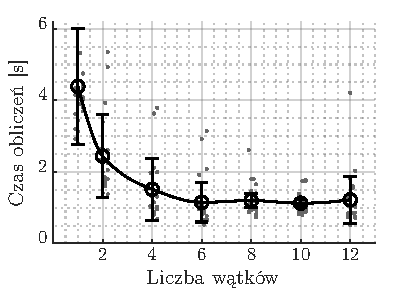
\includegraphics[width=1\linewidth]{grafiki/skalowalnosc_PSO_z1.pdf}
  \captionof{figure}{Test skalowalności algorytmu PSO na przykładzie optymalizacji zadania $1$. o $n = 20$ wymiarach. Użyto $100000$ cząstek.}
  \label{fig:skalowalnosc:PSO1}
\end{minipage} \hfill
\begin{minipage}[b]{\dimexpr.5\textwidth-1em}
  \centering
  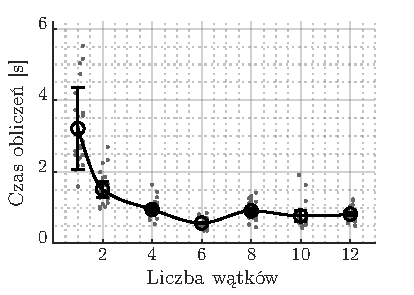
\includegraphics[width=1\linewidth]{grafiki/skalowalnosc_PSO_z2.pdf}
  \captionof{figure}{Test skalowalności algorytmu PSO na przykładzie optymalizacji zadania $2$. o $n = 10$ wymiarach. Użyto $100000$ cząstek.}
  \label{fig:skalowalnosc:PSO2}
\end{minipage}
\end{figure}

\begin{figure}[h]
\centering
\begin{minipage}[b]{\dimexpr.5\textwidth-1em}
  \centering
  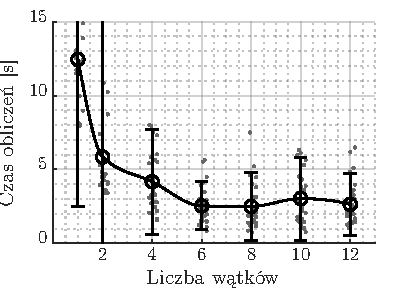
\includegraphics[width=1\linewidth]{grafiki/skalowalnosc_MC_z1.pdf}
  \captionof{figure}{Test skalowalności algorytmu MC na przykładzie optymalizacji zadania $1$. o $n = 10$ wymiarach. Użyto $100000$ cząstek.}
  \label{fig:skalowalnosc:MC1}
\end{minipage} \hfill
\begin{minipage}[b]{\dimexpr.5\textwidth-1em}
  \centering
  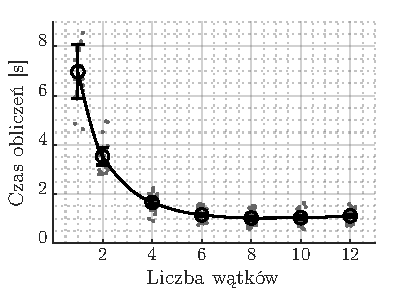
\includegraphics[width=1\linewidth]{grafiki/skalowalnosc_MC_z2.pdf}
  \captionof{figure}{Test skalowalności algorytmu MC na przykładzie optymalizacji zadania $2$. o $n = 4$ wymiarach. Użyto $10000$ cząstek.}
  \label{fig:skalowalnosc:MC2}
\end{minipage}
\end{figure}

\section{Porównanie trajektorii dla $n = 2$}

\section{Profil zbieżności algorytmów}

\section{Wnioski} 

\bibliography{PORR_sprawozdanie_1}{}
\bibliographystyle{plain}

\end{document}







